\documentclass{article}

% if you need to pass options to natbib, use, e.g.:
%     \PassOptionsToPackage{numbers, compress}{natbib}
% before loading neurips_2020

% ready for submission
% \usepackage{neurips_2020}

% to compile a preprint version, e.g., for submission to arXiv, add add the
% [preprint] option:
%     \usepackage[preprint]{neurips_2020}

% to compile a camera-ready version, add the [final] option, e.g.:
%     \usepackage[final]{neurips_2020}

% to avoid loading the natbib package, add option nonatbib:
\usepackage[nonatbib]{neurips_2020}

\usepackage[utf8]{inputenc} % allow utf-8 input
\usepackage[T1]{fontenc}    % use 8-bit T1 fonts
\usepackage{hyperref}       % hyperlinks
\usepackage{url}            % simple URL typesetting
\usepackage{booktabs}       % professional-quality tables
\usepackage{amsfonts}       % blackboard math symbols
\usepackage{nicefrac}       % compact symbols for 1/2, etc.
\usepackage{microtype}      % microtypography
\usepackage{float}
\usepackage{graphicx}

\title{Assignment 1 - Defining \& Solving RL Environments}

% The \author macro works with any number of authors. There are two commands
% used to separate the names and addresses of multiple authors: \And and \AND.
%
% Using \And between authors leaves it to LaTeX to determine where to break the
% lines. Using \AND forces a line break at that point. So, if LaTeX puts 3 of 4
% authors names on the first line, and the last on the second line, try using
% \AND instead of \And before the third author name.

\author{%
  Shaurya Mathur\thanks{Use footnote for providing further information
    about author (webpage, alternative address)---\emph{not} for acknowledging
    funding agencies.} \\
  Department of Computer Science\\
  Cranberry-Lemon University\\
  Pittsburgh, PA 15213 \\
  \texttt{smathur4@buffalo.edu} \\
  % examples of more authors
  % \And
  % Coauthor \\
  % Affiliation \\
  % Address \\
  % \texttt{email} \\
  % \AND
  % Coauthor \\
  % Affiliation \\
  % Address \\
  % \texttt{email} \\
  % \And
  % Coauthor \\
  % Affiliation \\
  % Address \\
  % \texttt{email} \\
  % \And
  % Coauthor \\
  % Affiliation \\
  % Address \\
  % \texttt{email} \\
}

\begin{document}

\maketitle

\begin{abstract}
  The report presents the code and results for the checkpoint for first assignment for CSE 546 - Reinforcement Learning. The goal of the assignment is to acquire experience in defining and solving RL environments, following
  Gymnasium standards. 
\end{abstract}

\section{Defining RL Environments}


\subsection{B.2 Traffic Light Control}
\textbf{Scenario:} A traffic light controller operates at a 4-way intersection. The goal is to minimize the average
wait time of cars by optimizing the traffic light switching strategy.


\subsection{Environment Setup}
\begin{itemize}
    \item \textbf{Grid Size:} 4x4 grid representing the intersection.
    \item \textbf{Cars:} Cars arrive at the intersection and must wait until they can move forward.
    \item \textbf{Goal:} Minimize the average wait time of cars at the intersection.
    \item \textbf{Actions:} Switch to Red, Green, or Yellow for each of the four directions.
    \item \textbf{Rewards:} 
    \begin{itemize}
        \item -1 for each second a car waits.
        \item +5 for each car that successfully passes through the intersection.
    \end{itemize}
    \item \textbf{Terminal State:} Defined by a maximum steps reached or a certain number of cars processed.
\end{itemize}

\subsection{Deterministic and Stochastic Environments}
\textbf{Deterministic Environment:}
\begin{itemize}
    \item The traffic flow is fixed, meaning cars arrive at fixed regular intervals from each direction.
    \item The timing and number of cars arriving at the intersection are predictable.
    \item Rewards: -1 per second a car waits, +5 for each car passing through the intersection.
\end{itemize}

\textbf{Stochastic Environment:}
\begin{itemize}
    \item The traffic flow is random, with cars arriving at irregular intervals.
    \item The reward function remains the same as in the deterministic setting.
    \item To simulate the arrival of cars on the intersection, the environment uses a probabilities for each directino totaling to 1. Each probability denotes the likelyhood of a car reaching the intersection in that direction.
\end{itemize}

\textbf{Other}
\begin{itemize}
    \item The environment has the capability to simulate different traffic conditions, such as heavy traffic during rush hour and light traffic during off-peak times.
\end{itemize}

\subsection{Environment Constraints}
\begin{itemize}
    \item \textbf{Legal Light Switching:} Traffic lights can't perform illegal action sequences such as switching to the same color twice or 1. Green 2. Yellow 3. Green. Environment terminates on an illegal action.
    \item \textbf{Light Timings:} Green traffic light stays and allows a single car to cross the intersection for 3 seconds and yellow light stays for 2 second.
    \item \textbf{Direction Constraints:} At a time step, only 1 direction can be green/yellow, all others will be red.
\end{itemize}


\section{Visualizations of Environment}

\subsection{Initial Environment State}

\begin{figure}[H]
    \centering
    \fbox{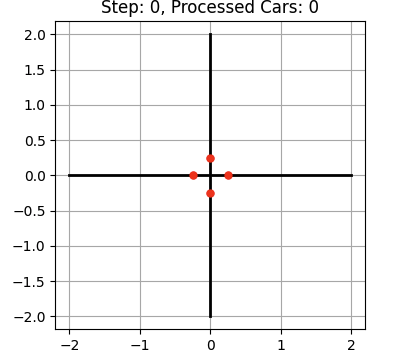
\includegraphics[width=7cm,height=7cm]{init.png}}
    \caption{Initial Environment State.}
\end{figure}

\subsection{Intermediate Environment States}

\begin{figure}[H]
    \centering
    \fbox{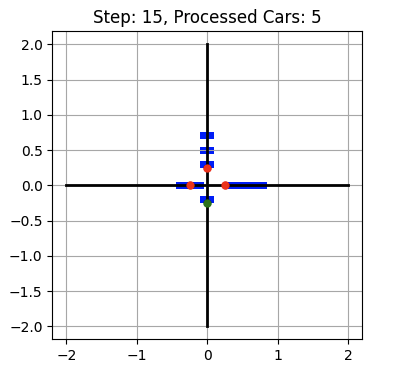
\includegraphics[width=7cm,height=7cm]{inter1.png}}
    \caption{Intermediate Environment State 1}
  \end{figure}

  \begin{figure}[H]
    \centering
    \fbox{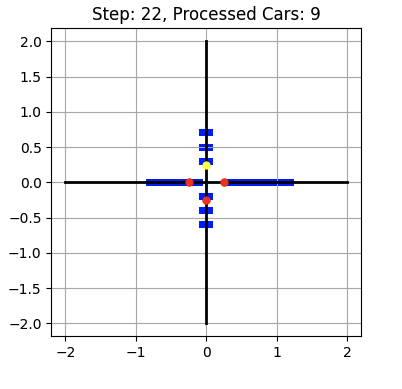
\includegraphics[width=7cm,height=7cm]{inter2.png}}
    \caption{Intermediate Environment State 2}
  \end{figure}

  \subsection{Terminal Environment State}

  \begin{figure}[H]
      \centering
      \fbox{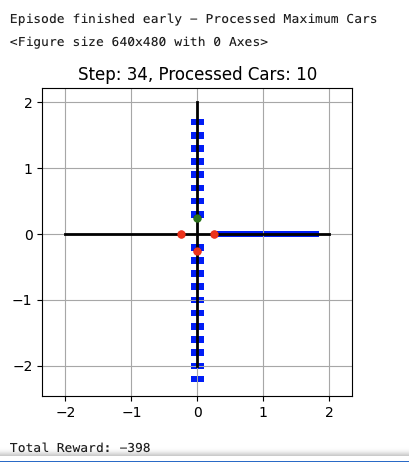
\includegraphics[width=7cm,height=7cm]{term.png}}
      \caption{Terminal Environment State}
  \end{figure}

\section{Safety in AI}

Ensuring safety in the traffic light control environment is crucial to prevent unrealistic or unsafe actions by the reinforcement learning (RL) agent. \\

\begin{itemize}
    \item We enforce constraints on the agent's action space, ensuring that it follows legal traffic light sequences (e.g., preventing a transition from Green directly back to Green without a Yellow phase). I have written a $\emph{\_is\_legal\_action}$ function which adds relevant constraints on the environment. 
    \item The state space is well-defined, ensuring the agent only operates within the valid 4x4 grid representing the intersection and the traffic light is changed only in one of the four directions. 
    \item The reward policy discourages unsafe behaviors—penalizing excessive wait times while rewarding efficient traffic flow. 
    \item In the stochastic environment, randomness in car arrivals is carefully controlled to avoid unrealistic congestion or deadlock scenarios. 
    \item The environment is capable of handling different traffic conditions, such as heavy traffic during rush hour and light traffic during off-peak times.
    \item Lastly, extensive testing and validation are performed to ensure that the trained agent generalizes well to various traffic conditions while maintaining safety constraints.\\
\end{itemize}


\section*{References}

\small

[1] https://gymnasium.farama.org/api/env/.

[2] Lecture slides.

[3] https://matplotlib.org/stable/index.html.

[4] https://docs.python.org/3/library/dataclasses.html

\end{document}